\chapter{بخش دوم}
در این بخش به طراحی کنترل کنترل‌کننده از خانواده  PID به کمک برنامه  \lr{PID tuner} متلب پرداخته شده است نمایی از دو کنترل‌کننده PI  و PIDF طراحی شده در فضای این برنامه به صورت زیر است:
\begin{figure}[H]
	\centering
	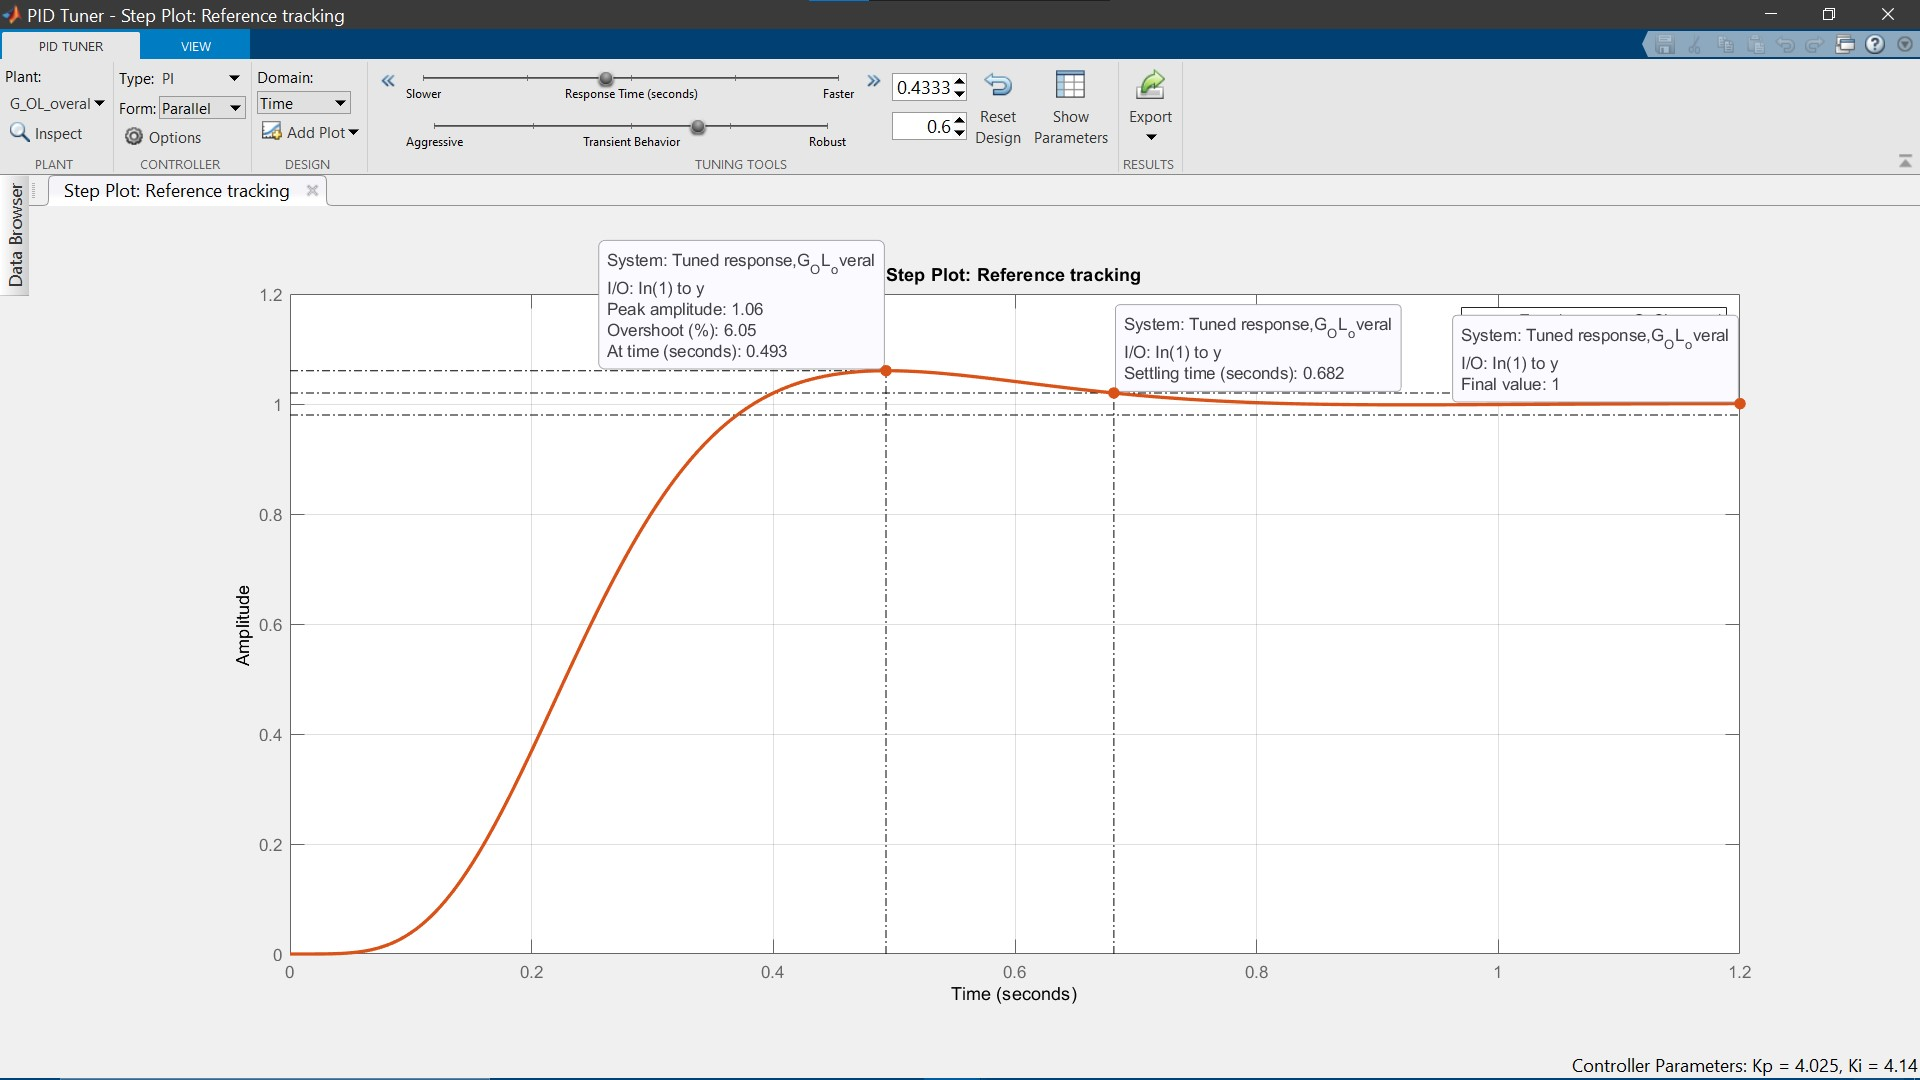
\includegraphics[width=12cm]{../Figure/P_II/controller_PIDtuner__partII_PI.jpg}
	\caption{کنترل‌کننده PI طراحی شده در برنامه \lr{PID tunner} متلب}
\end{figure}


پاسخ سیستم مداربسته به ازای ورودی مرجع پله واحد با دو کنترل‌کننده طراحی شده در این قسمت نیز به صورت زیر است:
\begin{figure}[H]
	\centering
	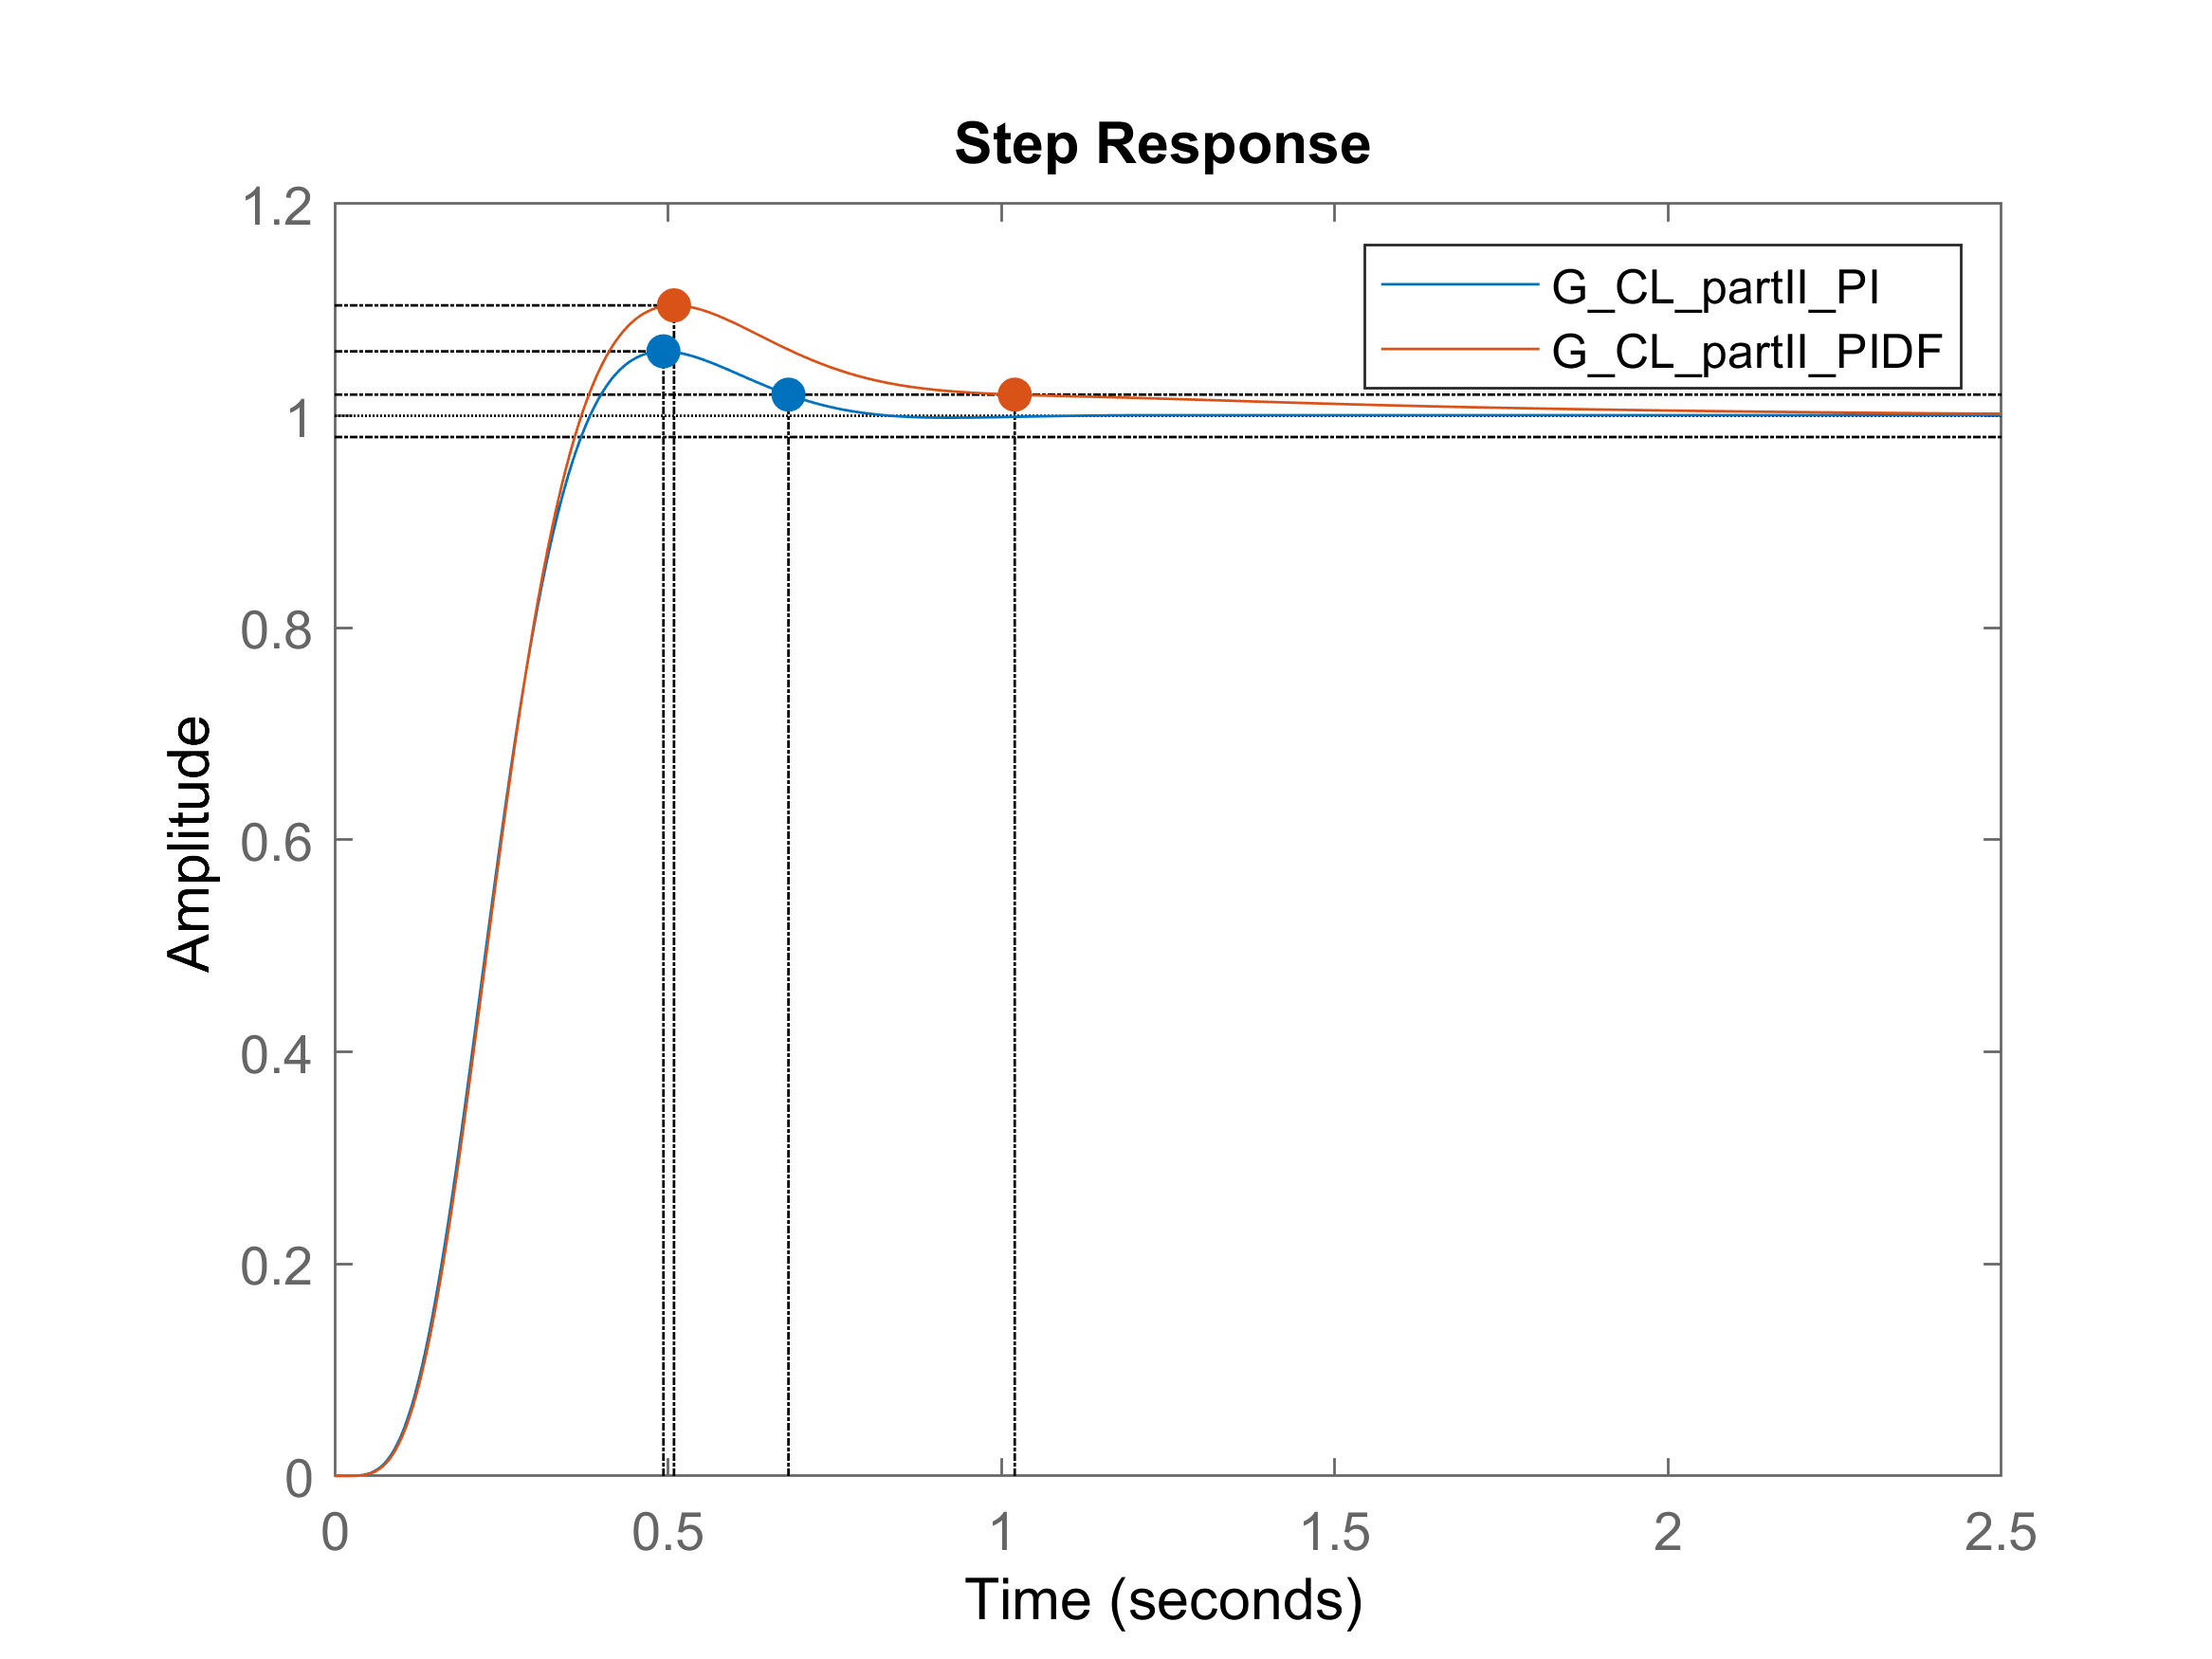
\includegraphics[width=12cm]{../Figure/P_II/PID_tunner.png}
	\caption{خروجی سیستم به ازای پله واحد با کنترل‌کننده PIDF و PI طراحی شده در برنامه \lr{PID tunner} متلب}
\end{figure}


همانطور که ملاحظه می شود مقدار اورشوت و زمان نشست کمتر از مقادیر موجود در خواسته های مسیله می باشد.
هم چنین با پیاده سازی کنترل‌کننده بالا در محیط سیمولینک همراه/بدون اشباع بر روی مدل غیر خطی شبیه سازی شده به صورت زیر:
\begin{figure}[H]
	\centering
	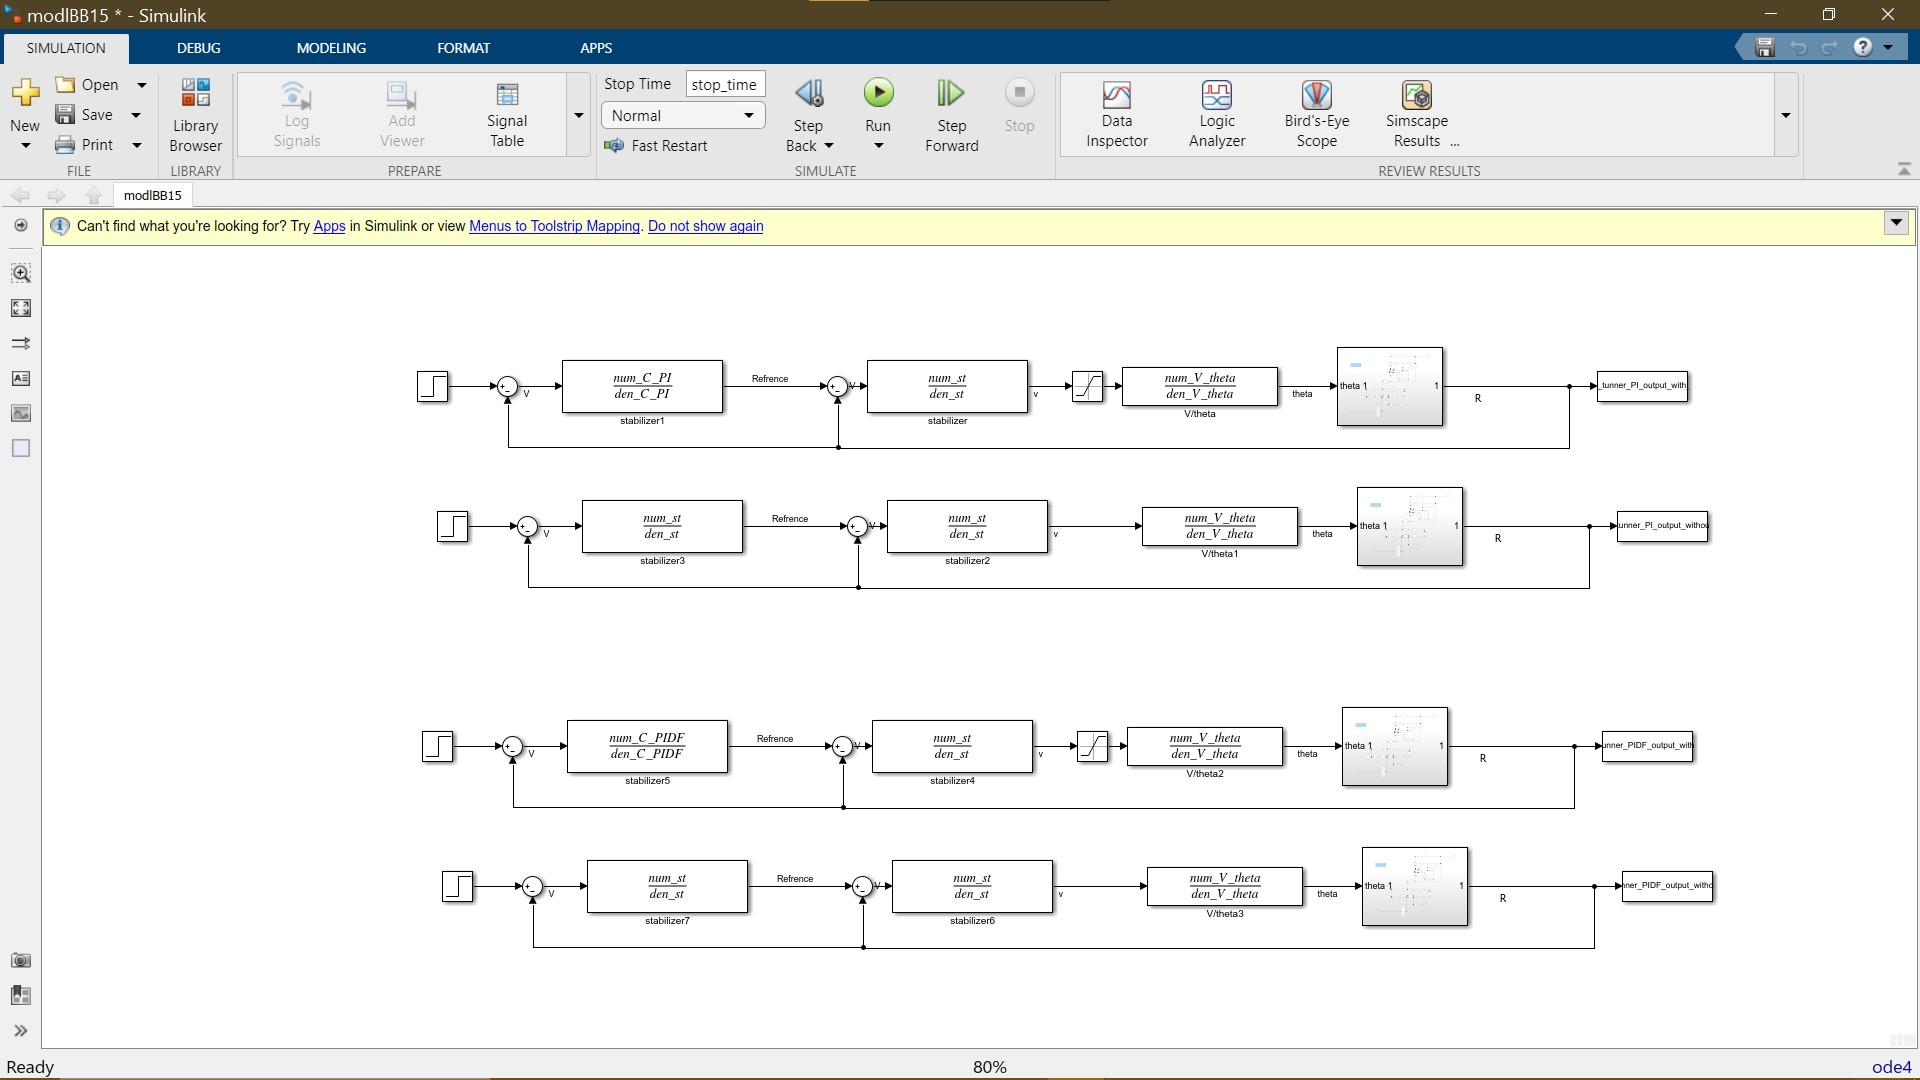
\includegraphics[width=12cm]{../Figure/P_II/simmechanic_simulink.jpg}
	\caption{پیاده سازی کنترل‌کننده طراحی شده به وسیله \lr{PID tunner} متلب بر روی مدل غیر خطی شبیه سازی شده}
\end{figure}

و پس از اجرای فایل سیمولینک برای هر کنترل‌کننده با اشباع ،خروجی به ازای ورودی مرجع 0.5 متر و نمایی از انیمیشن و شبیه سازی حرکت توپ به صورت زیر است:
%عکس: simmechanic1
%کپشن:نمایی از انیمیشن شبیه سازی حرکت توپ با کنترل‌کننده طراحی شده به وسیله PID tunner و همراه با بلوک اشباع
%عکس: simmechanic
%کپشن:پیاده سازی کنترل‌کننده طراحی شده به وسیله PID tunner  متلب بر روی مدل غیر خطی شبیه سازی شده
%همانطور که مشاهده می شود در مدل غیر خطی به دلیل اعمال بلوک اشباع عملگر،زمان نشست به حدود 150 ثانیه و اور شوت به حدود 35 درصد رسیده است.